\documentclass[a4paper,11pt]{report}
\usepackage[T1]{fontenc}
\usepackage[utf8]{inputenc}
\usepackage{lmodern}

\usepackage{hyperref}
\usepackage{graphicx}
\usepackage[english]{babel}

\usepackage{graphicx}
\usepackage{amsmath}

\usepackage{algorithm}
\usepackage{algorithmic}

\usepackage{listings} % package for listing parts of code
\usepackage{todonotes}
\usepackage{subcaption}


\renewcommand*\footnoterule{}

\makeatletter
\renewcommand{\@chapapp}{}% Not necessary...
\newenvironment{chapquote}[2][2em]
  {\setlength{\@tempdima}{#1}%
   \def\chapquote@author{#2}%
   \parshape 1 \@tempdima \dimexpr\textwidth-2\@tempdima\relax%
   \itshape}
  {\par\normalfont\hfill--\ \chapquote@author\hspace*{\@tempdima}\par\bigskip}
\makeatother




% Book's title and subtitle
\title{\Huge \textbf{High Performance Computing with Python} \vspace{4mm} \\ \huge Final Report}
% Author
% \author{\textsc{First-name Last-name}\footnote{email address}}
\author{\textsc{Ayisha Ryhana Dawood} \\ \vspace{3mm}\text{5653447}  \\
\vspace{3mm}\text{dawooda@informatik.uni-freiburg.de}}


\begin{document}

\makeatletter
    \begin{titlepage}
        \begin{center}
            
\includegraphics[width=0.5\linewidth]{logos/Uni_Logo-Grundversion_E1_A4_CMYK.eps}\\[4ex]
            {\huge \bfseries  \@title }\\[2ex] 
            {\LARGE  \@author}\\[30ex] 
            {\large \@date}
        \end{center}
    \end{titlepage}
\makeatother
\thispagestyle{empty}
\newpage



\tableofcontents


\chapter{Introduction}
The Lattice Boltzmann method provides a simulation technique that uses a 
density distribution to model fluid flow including turbulence, multi-component and multi-phase
flows as well as additional applications \cite{lbm_intro}. The report starts by discussing the Boltzmann Transport Equation and the different components of the method that are important from an implementation perspective.

Fluid mechanics deals with the movements and interactions of fluids and are of high importance in many fields of study and industry. Experimentation with fluids on a large scale can be challenging. Simulation of experiments provides a solution to this problem. As the scale of experiments increase, the computational technologies used in the simulations need to be upgraded to handle the complexities. 

High Performance Computing (HPC) is the use of advanced computational techniques like parallel processing, multi-core processors, GPU accelerations, cluster computing, super-computing and others to achieve efficiency and accuracy in solving complex problems. C and FORTRAN are popular programming language used to achieve HPC due to the ability to write highly optimized code with control over memory management and hardware interactions. Python, well known for its simplicity and wide use in AI/ML, is also being used for HPC through libraries like NumPy. This allows for high-level programming while still being able to interface libraries implemented in C and FORTRAN.

In this report, HPC concepts are realized using Python. The Boltzmann Transport Equation is simulated without HPC for different initial configurations and boundary conditions to validate the implementation incrementally. Finally, the Sliding Lid induced cavity is simulated using HPC elements like spatial domain decomposition (splitting the lattice grid into sub-domains to be processed independently) and the MPI (\texttt{mpi4py} package) for message passing between the sub-domains. The performance across implementations with multiple processor counts are observed. The simulation is repeated for various initial configurations and the performance is noted.

The results in this report can be reproduced by the code base and instructions of the associated GitHub repository \footnote{The code is available at: \url{https://github.com/AyishaR/HPC-fluid-mechanics-with-python}}

\chapter{Lattice Boltzmann Method}
The Lattice Boltzmann method is a computational technique to approximate fluid behaviour by simulating the trajectory of discrete particles and their interactions on a lattice grid. The approximation is done by breaking down the fluid flow into discretized steps - streaming (movement of the particles along the axes of the lattice), collision (interaction of particles with one another) and boundary conditions (behaviour of the particles at the boundaries of the lattice grid).

\section{The Boltzmann Transport Equation (BTE)}
The Boltzmann equations are discretizations of the kinetic equations of Lattice Gas Cellular Automaton (LGCA) \cite{wolf_gladrow_lgca_lbm}.
\begin{equation}
\frac{\partial f}{\partial x} +\mathbf{v}{\nabla f}=Q
\end{equation}
Here, Q is the collision integral that models complex particle interactions and scattering processes. The BGK approximation is an alternate low-level discretization of the original Boltzmann equation that pushes the system towards an equilibrium.

\begin{equation}\label{eq:LBE}
f_i(\mathbf{r}+\mathbf{c}_i\cdot\Delta t,t+\Delta t)-f_i(\mathbf{r},t)=
 -\frac{f_i(\mathbf{r},t)-f_i^\text{eq}(\mathbf{r},t)}  \tau 
\end{equation}

\begin{equation}\label{eq:LBE_2}
\underbrace{f_i(\mathbf{r}+\mathbf{c}_i\cdot\Delta t,t+\Delta t)-f_i(\mathbf{r},t)}_{streaming}=
\underbrace{-\omega \left( f_i(\mathbf{r},t)-f_i^\text{eq}(\mathbf{r},t) \right)}_{collision}
\end{equation}

The collision term is calculated using the equilibrium state and the relaxation time constant $\tau$. The system is driven into global equilibrium at the rate $\Omega$. This simplified model does not take into consideration the external forces on the system as the inter-atomic processes being modelled occur instantaneously compared to the changes induced by external forces. The density and velocity of the fluid characterized by the particle probability density $f(\mathbf{r},\mathbf{v},t)$ is given as follows,

\begin{equation}
    \rho (\mathbf{r}, t) =  \int f\left(\mathbf{r},\mathbf{v},t\right) d\mathbf{v}
\end{equation}

\begin{equation}
    \mathbf{u}(\mathbf{r}, t) = \frac1 {\rho (\mathbf{r}, t)} \int \mathbf{v} f\left(\mathbf{r},\mathbf{v},t\right) d\mathbf{v}
\end{equation}


The BTE can now be used to simulate fluid flow and calculate the state of the system at time step $t+\Delta t$ given the state at time $t$.

\begin{equation}\label{eq:LBE_3}
f_i(\mathbf{r}+\mathbf{c}_i\cdot\Delta t,t+\Delta t) = f_i(\mathbf{r},t)
-\omega \left( f_i(\mathbf{r},t)-f_i^\text{eq}(\mathbf{r},t) \right)
\end{equation}

\section{Lattice Grid}
Lattice grids represent the discretized domain where the above equations are used to simulate fluid flow. The lattice structures are described by the notation 

\begin{center}
    \textbf{DdQq}
\end{center}

where the character D indicates dimensionality and Q indicates velocity directions. d and q are integers that represent the number of dimensions and number of discrete velocity directions respectively.

Higher values of d and q lead to computationally expensive simulations while lower dimensions and fewer vector directions affect accuracy of the simulation. In this report, the D2Q9 lattice is used, i.e., 2D fluid flows are simulated with 9 discrete velocity vectors as a balance between accuracy and computational efficiency.

\begin{figure}[h!]
  \begin{center}
   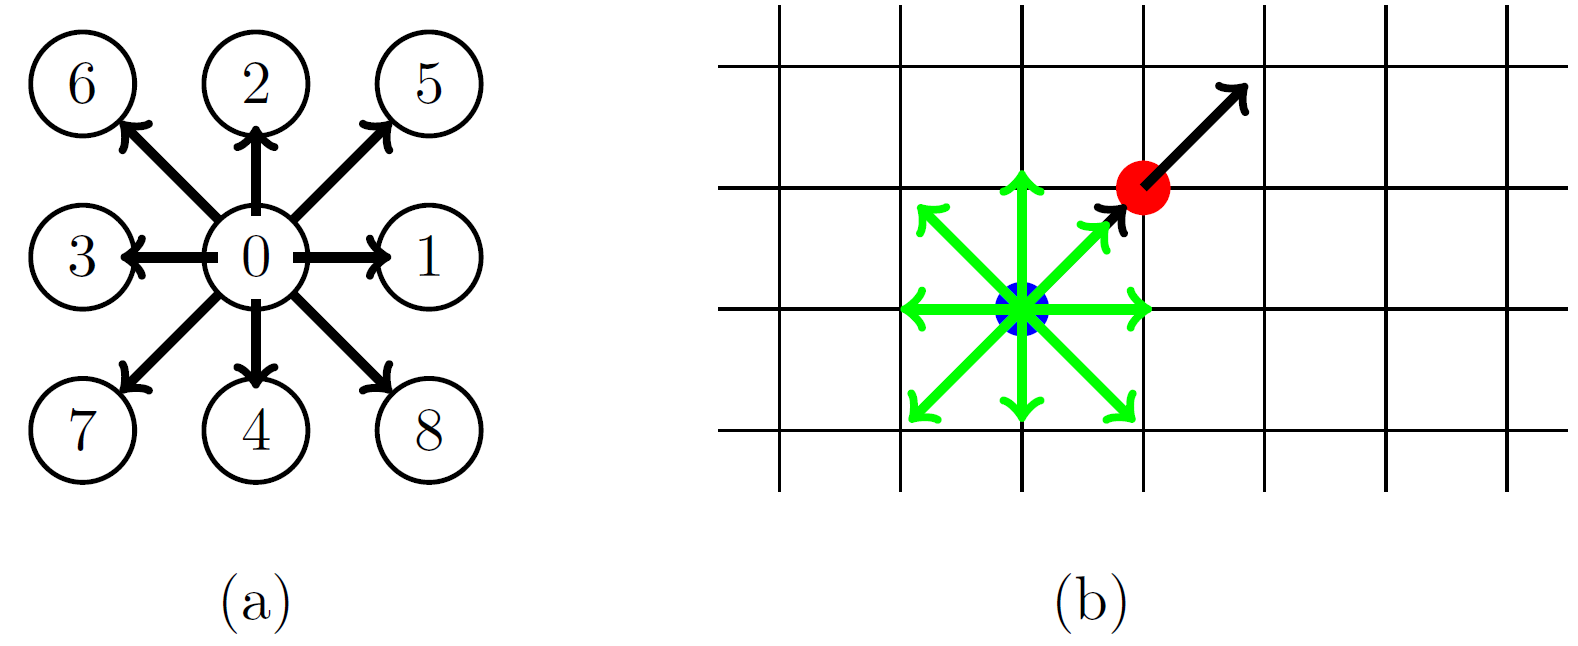
\includegraphics[width=10cm]{logos/Gitter_LBM.png}
   \caption{(a) 9 discrete velocity directions. (b) D2Q9 lattice grid showing velocity vectors of one particle. \cite{Pastewka2019HPCWP}}
  \label{fig:mesh}
  \end{center}
\end{figure} 

\section{Streaming}
\label{sec:streaming}
The discretization of velocity space results in velocity sets that define movements along the prescribed directions. Streaming is the shift of lattice velocity in these directions for $\Delta t$. 

For a node \textbf{r} in a D2Q9 lattice, the velocity sets are described by a $9\times 2$ ($q\times d$) matrix as follows,

\begin{equation}
c =  \begin{pmatrix}
 0 & 1 & 0 & -1 & 0 & 1 & -1 & -1 & 1\\
 0 & 0 & 1 & 0 & -1 & 1 & 1 & -1 & -1
 \end{pmatrix} ^{T} 
\end{equation}

When $\Delta x$, $\Delta y$ and $\Delta t$ are unity, the discretized probability density function $f_i$ of node \textbf{r} will be shifted along the lattice with velocity $c_i$ to the immediate adjacent node in the specified directions.

\section{Collision}
\label{sec:collision}
Collision describes the interaction between particles on the lattice grid. It is discretized by a relaxation time approximation that implies that system locally relaxes towards an equilibrium distribution $f^{eq}$.

The equilibrium state depends on the local variables - the local density $\rho(\mathbf{r})$ and the local average velocity $\mathbf{u}(\mathbf{r})$.

\begin{equation}
    \rho (\mathbf{r}) =  \sum_i f_i
\end{equation}

\begin{equation}
    \mathbf{u}(\mathbf{r}) = \frac1 {\rho (\mathbf{r})} \sum_i {c_i f_i\left(\mathbf{r}\right)}
\end{equation}

\begin{equation}
f^{eq}_i(\rho(\mathbf{r}),\mathbf{u}(\mathbf{r})) = w_i \rho(\mathbf{r})\left[1+3 c_i \cdot \mathbf{u}(\mathbf{r})+ \frac9 2 (c_i \cdot \mathbf{u}(\mathbf{r}))^2 - \frac3 2 |\mathbf{u}(\mathbf{r})|^2\right] 
\end{equation}

$w_i$ is a $1\times 9$ ($1\times q$) matrix describing the weights of the particle interactions in the velocity directions.

\begin{equation}
    w_i=(\frac4 9,\frac1 9,\frac1 9,\frac1 9,\frac1 9,\frac1 {36},\frac1 {36},\frac1 {36},\frac1 {36})
\end{equation}


\section{Boundary conditions}
\label{sec:boundary}
Boundary conditions define the behaviour of particles at the boundary nodes of the lattice grid. The sequence of execution with respect to streaming and collision operations is crucial. All boundary conditions discussed below, except pressure gradient are applied after the streaming step. These conditions are applied to the particle probability density function $f_i$ and not the physical variables $\rho$ and $\mathbf{u}$. \\

\noindent The boundaries of the lattice grids can be implemented in two ways: \cite{liu_zhou_2014}
    \begin{enumerate}
        \item Dry Node 
        
        The boundaries are located on the link between 2 nodes, i.e., the node is part of the grid where there is no fluid pressure and act as an interface between surfaces depicted by nodes on either side.

        \item Wet Node

        The boundaries are present on the lattice node, i.e., the node is located where the fluid is present.
    \end{enumerate}
\noindent In this implementation, dry nodes are used because of they are simpler to handle.

\subsection{Periodic Boundary Conditions (PBC)}
Periodic boundary conditions are used to implement symmetric conditions where the fluid that leaves the lattice grid through one boundary, re-enters through the opposite side during the streaming operation. In addition to the lattice shift during streaming, the following condition needs to be satisfied. \cite{Succi_10.1093/oso/9780199592357.001.0001}
\begin{equation}
    f_i(\mathbf{x_0}, t) = f_i(\mathbf{x_{N-1}}, t)
\end{equation}
where $x_0$ and $x_{N-1}$ are the first and last nodes in the physical domain of a lattice grid with N nodes. This is easily achieved using the \texttt{np.roll} function in the \texttt{numpy} package.

\subsection{Rigid wall (Bounce back)}
Bounce back conditions are implemented to simulate interaction of fluid particles with a rigid wall. The assumption is that the velocity vectors facing the wall perfectly bounce back ($180^0 $) after streaming. For example, consider a wall on the left boundary of a lattice grid. The probability density values of channels facing the wall are $f_6, f_3, f_7$. After streaming, the channels $f_8, f_1, f_5$ are overwritten by the values in $f_6, f_3, f_7$. 

For the generic implementation, $f^{\star}$ is the probability density before streaming, and $\overline{i}$ is the channel opposite to $i$. \cite{Succi_10.1093/oso/9780199592357.001.0001}
\begin{equation}
    f_{\overline{i}}(\mathbf{x_b}, t+\Delta t) = f^{\star}_i(\mathbf{x_b}, t)
\end{equation}
\subsection{Moving wall}
Moving walls along a fluid surface contribute to the momentum of the fluid. In addition to bounce back, the velocity of the wall $u_w$ is also incorporated to the equation. \cite{Succi_10.1093/oso/9780199592357.001.0001}
\begin{equation}
    f_{\overline{i}}(\mathbf{x_b}, t+\Delta t) = f^{\star}_i(\mathbf{x_b}, t) - 2 w_i \rho_w \frac{\mathbf{c_i} \cdot \mathbf{u_w}} {c^2_s}
\end{equation}
Here, $c_s = \frac{1}{\sqrt{3}}$ is the speed of sound and $\rho_w$ is the density of the wall.

The Sliding Lid induced cavity simulation involves a moving wall on the top boundary of the lattice. To simplify calculation of channel populations $f_7, f_4, f_8$, the following implementation was used \cite{Mohamad2019}. $\rho_N, u_N, v_N$ are the density, horizontal velocity and vertical velocity of the top boundary.
\begin{equation}
\begin{aligned}
    \rho_N &= \frac1 {1+v_N} \left[f_0+f_1+f_3+2\left(f_2+f_6+f_5\right)\right] \\
    f_4 &= f_2 - \frac2 3 \rho_N v_N \\
    f_7 &= f_5 + \frac1 2 \left( f_1 - f_3 \right) - \frac1 6 \rho_N v_N - \frac1 2 \rho_N u_N \\
    f_8 &= f_6 + \frac1 2 \left( f_3 - f_1 \right) - \frac1 6 \rho_N v_N + \frac1 2 \rho_N u_N
\end{aligned}
\end{equation}

\subsection{Pressure Gradient}
A pressure variation of $\Delta p$ is applied between the inlet ($p_{in}$) and outlet ($p_{out}$). Pressure and density are related through the ideal gas equation of state. 
\begin{equation}
    p = c^2_s \rho
    \label{eq:pressure_density}
\end{equation}
with  $c^2_s$=1/3  in lattice units.

The lattice grid is created with a buffer layer of one node. $x_0$ and $x_{N+1}$ are the buffer nodes for lattice with size N between inlet and outlet. The boundary conditions are applied before the streaming step. \cite{Succi_10.1093/oso/9780199592357.001.0001}

\begin{equation}
    \begin{aligned}
        f^{\star}_i(x_0,y,t) &= f^{eq}_i(\rho_{in}, \mathbf{u_N}) + \left( f^{\star}_i(x_N,y,t) - f^{eq}_i(x_N,y,t)\right) \\
        f^{\star}_i(x_{N+1},y,t) &= f^{eq}_i(\rho_{out}, \mathbf{u_N}) + \left( f^{\star}_i(x_1,y,t) - f^{eq}_i(x_1,y,t)\right)
    \end{aligned}
\end{equation}

\chapter{Implementation and Code Snippets}
This section discusses the implementation details and few code snippets to explain them better. 
\section{Lattice grid visualization}
The Lattice Bolztmann Method models particles on the lattice grid by discretization. Visualizing the results is an easy way to verify that the simulations are working as intended. This includes density plots, streamlines indicating the velocity, decay plots and others. The density plots in this report do not show the buffer layers. The x-axis is horizontal and the y-axis is vertical. The velocity vector directions are same as in Figure \ref{fig:mesh}.

\begin{figure}[h]
  \begin{center}
   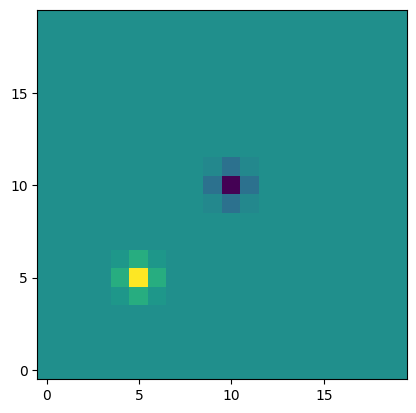
\includegraphics[height=4cm]{images/sample_lattice.png}
   \caption{Density plot of a sample D2Q9 lattice grid of grid size 20x20 with one time step propagation and relaxation.}
  \label{fig:sample_lattice}
  \end{center}
\end{figure} 

\section{Code Elements}
The \texttt{numpy} package is extensively used for all array data structures. The numpy array \texttt{f} with shape \texttt{(9,nx,ny)} stores the  probability density across all channels, \texttt{rho} with shape \texttt{(nx,ny)} stores the density values and \texttt{u} with shape \texttt{(2,nx,ny)} stores the velocity values $u_x$ and $u_y$ for each node on the lattice grid.

\section{Algorithmic Workflow} 
Every simulation follows a workflow that comprises a consistent set of components. 
It begins with parsing the command-line arguments to configure the parameters of the simulation. 
Each parameter has a default value configured that can be over-written by passing custom values through the command line. 
Some parameters that are common across all simulations include sizeof the grid (\texttt{-nx, -ny}), omega (\texttt{-o}), time steps (\texttt{-nt}) and the interval to log values for visualization or post-processing (\texttt{-nt\_log}). 
Few simulation specific parameters can also be configured like inlet and outlet density (\texttt{-rho\_in and -rho\_out}) for Poiseuille Flow simulation. The arguments can also be used to trigger specific types of execution like comparison of fluid flow with different initial velocities or different omega values.

The next step is the simulation. It begins with streaming (propagation), followed by applying boundary conditions specific to the scenario. In case of pressure gradients, the boundary condition is applied before streaming. This is followed by collision (relaxation), which models the interaction between particles as the system locally relaxes towards equilibrium. \cite{Krueger2017TheLB}

\begin{algorithm}
  \caption{Lattice Boltzmann Method}
  \label{alg:lbm}
  \begin{algorithmic}
    \STATE f: ($9, N_x, N_y$)
    \STATE $\rho$: ($N_x, N_y$) Initial density $\rho_0$
    \STATE u: ($2, N_x, N_y$) Initial velocity $u_0$
    \STATE c: ($9, 2$)
    \STATE w: ($1, 9$)
    \STATE nt: Number of timesteps

  \end{algorithmic}
  \begin{algorithmic}[1]
    \STATE $\rho\left(0\right)=\rho_0$; $u\left(0\right)=u_0$
    \FOR{$i = 1$ to $nt$}
      \STATE $f'(t + 1) = streaming(f(t))$ \begin{flushright}Section \ref{sec:streaming}\end{flushright}
      \STATE $f'(t + 1) = boundary_handling(f'(t+1))$ \begin{flushright}Section \ref{sec:boundary}\end{flushright}
      \STATE $f^{eq}(t) = equilibrium(\rho'(t+1),u'(t+1))$ 
      \STATE $f(t+1) = f'(t+1) + \omega(f^{eq}(t+1) - f'(t+1))$ \begin{flushright}Section \ref{sec:collision}\end{flushright}
    \ENDFOR
  \end{algorithmic}
\end{algorithm}


The simulation is followed by plotting relevant graphs. The density of the lattice grid is most common. Flow specific plots like velocity profile or density variations are plotted and compared to analytical values where relevant.

\section{Parallel implementation}
The parallellization of LBM is done using spatial domain decomposition. The lattice grid is divided into $n$ non-overlapping sub-domains for independent processing in a computing unit or processor. The sub-domains are adjacent parts of the lattice grid and need to communicate the channel populations periodically. The final populations of the channels in each sub-domain also needs to be consolidated at the end of the simulation from the different processing units to be presented as a full lattice grid. This is achieved by the message passing interface (MPI).

The number of computing units \texttt{size} and the dimensions of the lattice grid $N_x \times N_y$ are used to calculate the number of sub-domains along each axis \texttt{sects\_X} and \texttt{sects\_Y}. These, in addition to the \texttt{rank} of the computing unit are used to calculate the coordinates of the sub-domain of lattice grid processed by it. 

Each sub-domain has a buffer layer of size 1 that is communicated with sub-domains on all sides. This communication is done through the \texttt{Sendrecv} function in \texttt{mpi4py}. In one communication, data from the top non-buffer layer is sent to the last buffer layer of the sub-domain on top and similar data vector is received from the sub-domain below into the last buffer layer of the current sub-domain (Communication from Rank 0 to rank 1 in Figure \ref{fig:mpi-communication}). This way the data vectors are exchanged in pairs along each of the 4 directions - up, down, left and right. 

\begin{figure}[h]
  \begin{center}
  \rotatebox{90}{
   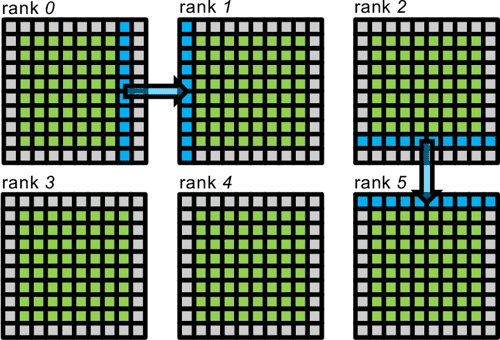
\includegraphics[height=5cm]{images/mpi-communication.png}
   }
   \caption{Spatial domain decomposition and visualization of the Message Passing Interface (MPI). The green cells are the physical domain and the grey cells are the buffer layer. \cite{Pastewka2019HPCWP}}
  \label{fig:mpi-communication}
  \end{center}
\end{figure} 


\chapter{Simulation results}


\section{Validating LBM components}
The realization of Sliding Lid induced cavity by parallelization starts with implementing and understanding the different elements of the Lattice Boltzmann method incrementally. This makes it easier to comprehend the concept and avoid errors in developing the simulation code.
\subsection{Shear Wave Decay}
Shear Wave Decay refers to the attenuation of the shear waves propagated through a material. The fluid system is initialized with a sinusoidal velocity or sinusoidal density and the behaviour of the system is monitored across time steps. The lattice grid has Periodic Boundary Conditions on all four boundaries.

Sinusoidal velocity is simulated with the following initial conditions for density and velocity.
\begin{equation}
    \begin{aligned}
        \rho \left( \mathbf{r}, 0 \right) &= 1\\
        \mathbf{u} \left( \mathbf{r}, 0 \right) &= \begin{pmatrix} {\varepsilon sin\left( \frac{2 \pi y} {L_y}\right) } \\ 0 \end{pmatrix} 
    \end{aligned}
\end{equation}

As $t \rightarrow  \infty $, the velocity decays to 0 as the system reaches equilibrium. 

\begin{figure}[h!]
  \begin{center}
   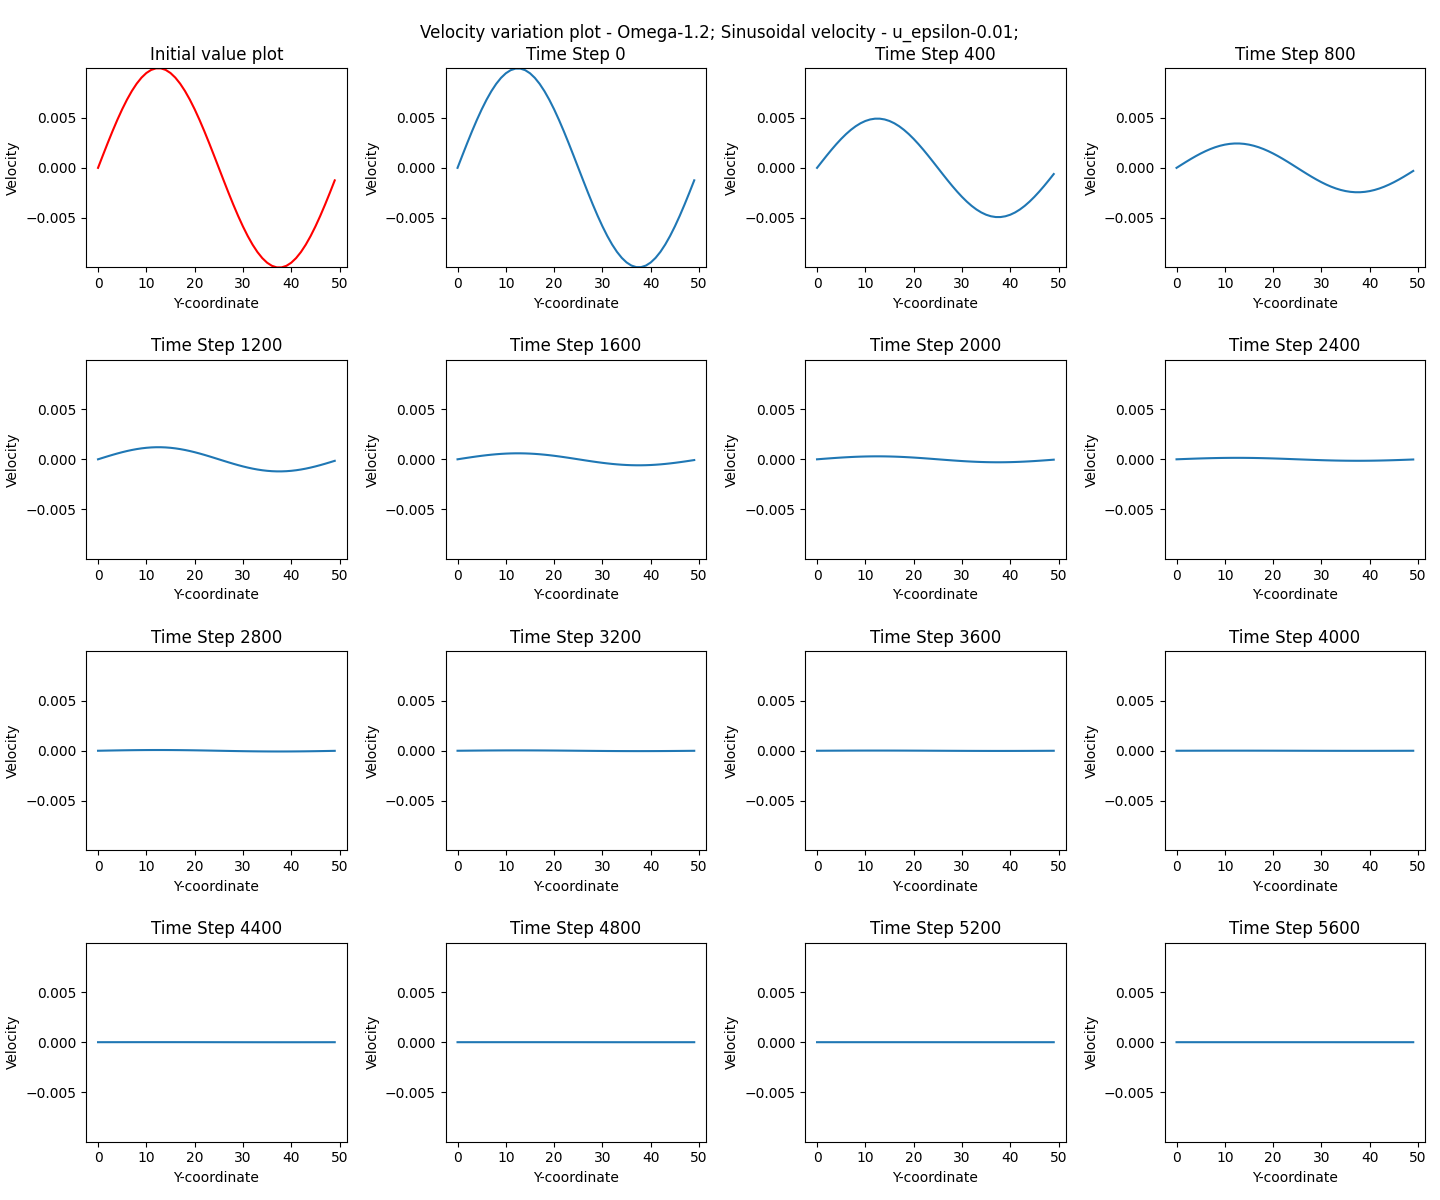
\includegraphics[width=0.8\textwidth]{HPC_report/images/shear_wave_decay/sinusoidal_velocity/Decay-Y-coordinate-Velocity.png}
   \caption{Time evolution of velocity at x=25 in lattice grid size 50x50 with configuration $\omega = 1.2, \varepsilon = 0.01$ and Periodic Boundary Conditions}
  \label{fig:swd_sv_ind}
  \end{center}
\end{figure} 

\begin{figure}[h!]
  \begin{subfigure}{0.3\textwidth}
        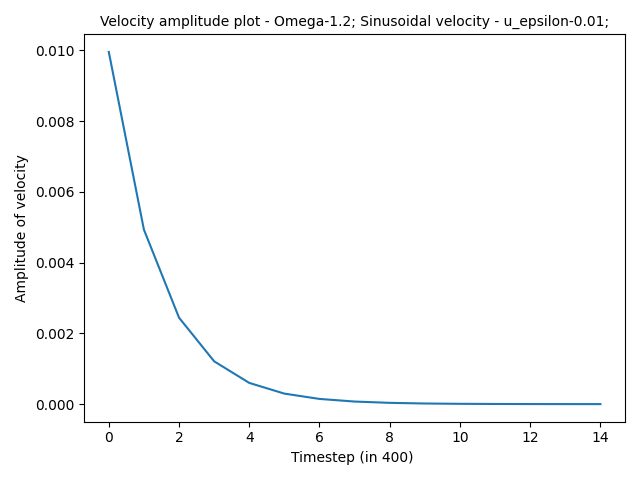
\includegraphics[width=\linewidth]{HPC_report/images/shear_wave_decay/sinusoidal_velocity/Amplitude-Timestep (in 400) -Amplitude of velocity.png}
        \captionsetup{font=small}
        \caption{Amplitude of velocity along the Y-axis}
    \end{subfigure}
    \begin{subfigure}{0.3\textwidth}
        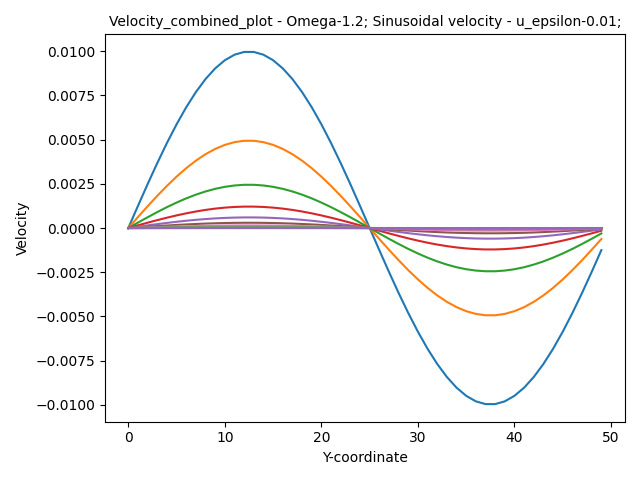
\includegraphics[width=\linewidth]{HPC_report/images/shear_wave_decay/sinusoidal_velocity/Combined_plot-Y-coordinate-Velocity.png}
        \captionsetup{font=small}
        \caption{Time evolution of velocity}
    \end{subfigure}
    \begin{subfigure}{0.3\textwidth}
        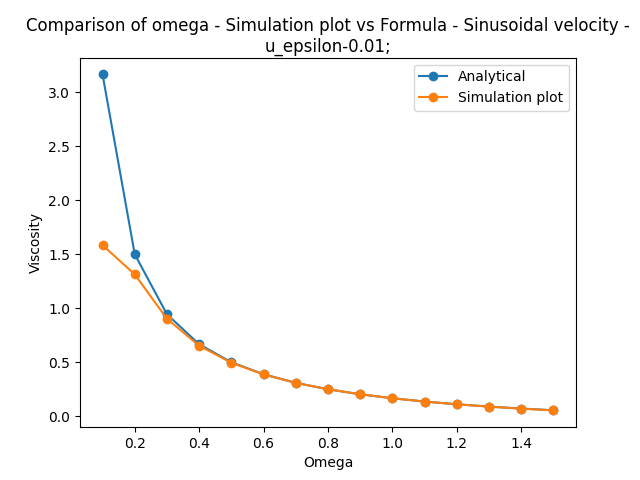
\includegraphics[width=\linewidth]{HPC_report/images/shear_wave_decay/Omega_comparison_Sinusoidal velocity_0.1_1.5_15.png}
        \captionsetup{font=small}
        \caption{Analytical vs simulated viscosity}
        \label{fig:v_ac}
    \end{subfigure}
    \caption{Values for x=50 in lattice grid size 100x100 with configuration $\omega = 1.2$, Sinusoidal velocity with $\varepsilon = 0.01$ and Periodic Boundary Conditions}
\end{figure} 

Sinusoidal density is simulated with the following initial conditions for density and velocity.
\begin{equation}
    \begin{aligned}
        \rho \left( \mathbf{r}, 0 \right) &= \rho_0 + \varepsilon sin\left( \frac{2 \pi x} {L_x}\right) \\
        \mathbf{u} \left( \mathbf{r}, 0 \right) &= 0
    \end{aligned}
\end{equation}

As $t \rightarrow  \infty $, the density decays to 0 as the system reaches equilibrium. But unlike velocity, the density oscillates before eventually reaching 0.

\begin{figure}[h!]
  \begin{center}
   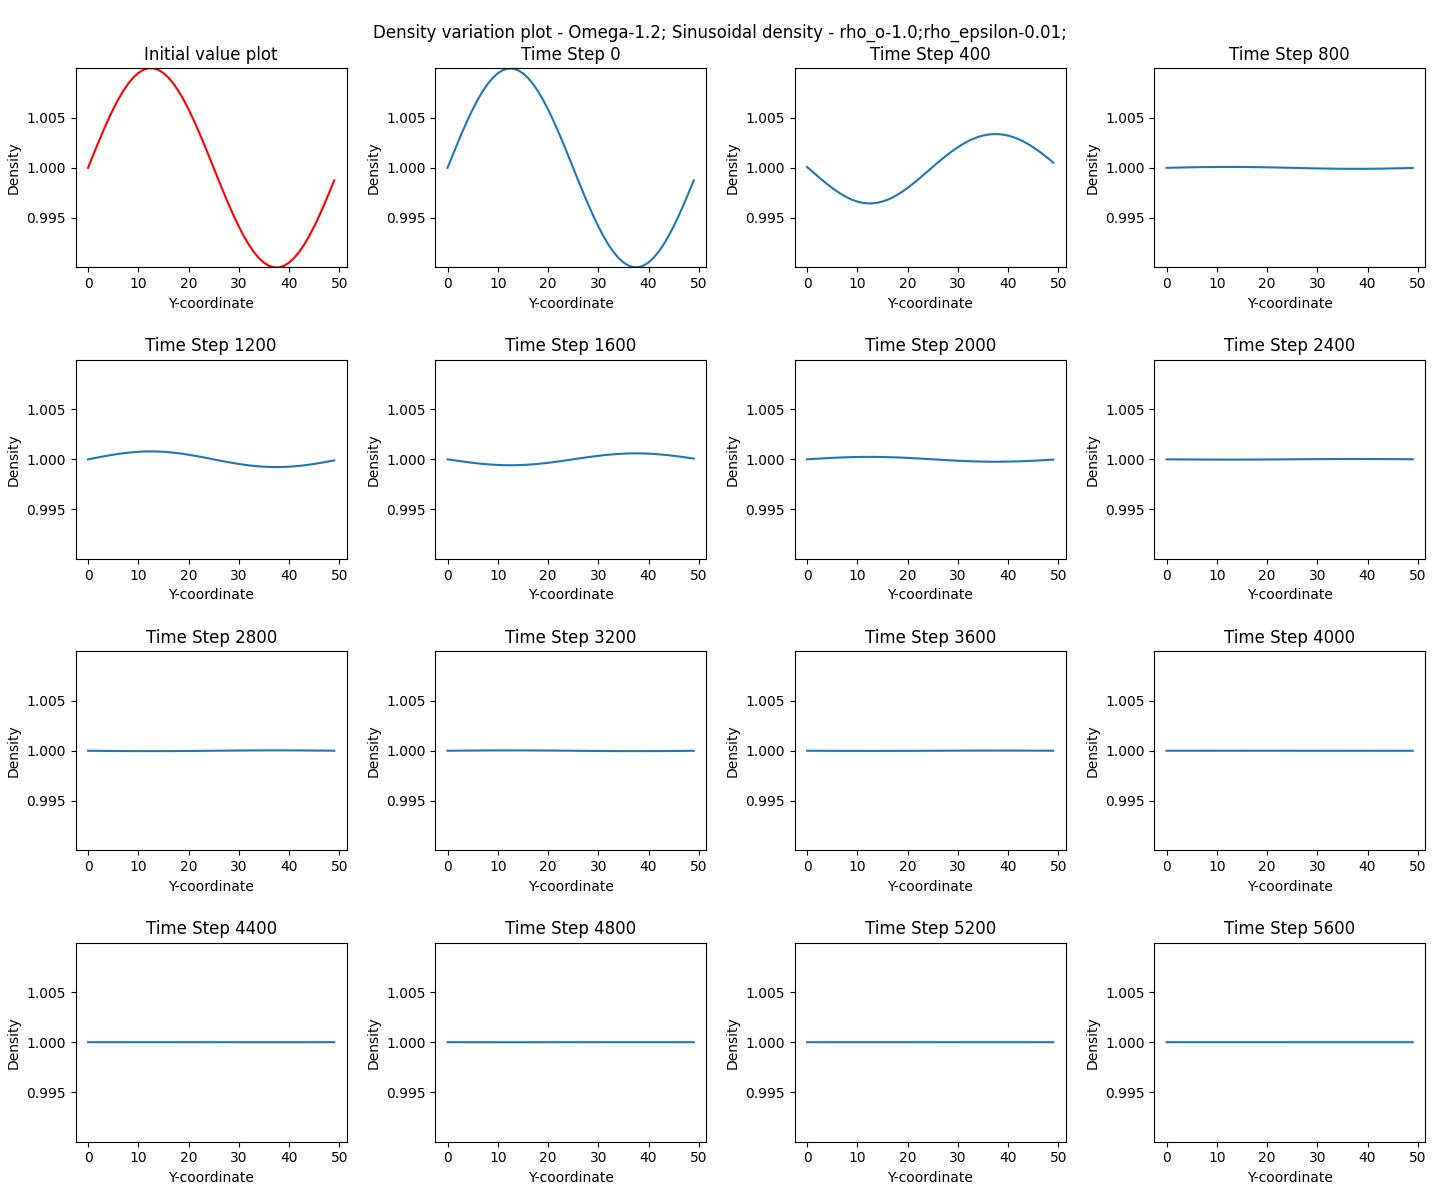
\includegraphics[width=0.8\textwidth]{HPC_report/images/shear_wave_decay/sinusoidal_density/Decay-Y-coordinate-Density.png}
   \caption{Time evolution of density at x=25 in lattice grid size 50x50 with configuration $\omega = 1.2, \rho_0 = 1$ and $\varepsilon = 0.01$ and Periodic Boundary Conditions}
  \label{fig:swd_sd_ind}
  \end{center}
\end{figure} 


The same is repeated for values of omega ranging from 0.1 to 1.5. In each simulation, the viscosity is measured in two ways. One is the simulated viscosity calculated from the velocity values in different time steps. Other is the measured viscosity calculated by assuming that the initial configuration fulfills the Stokes flow condition in Equation \ref{eq:stokes}. This gives Equation \ref{eq:viscosity} for analytical kinematic viscosity \cite{Krueger2017TheLB}. The plots in Figure \ref{fig:v_ac} and Figure \ref{fig:d_ac} compare the viscosity calculated by the two methods.
\begin{equation}
    \frac{\partial \mathbf{u}} {\partial t} = \nu \Delta \mathbf{u}
    \label{eq:stokes}
\end{equation}

\begin{equation}
    \nu = c^2_s \left( \frac1 {\omega} - \frac1 2 \right)
    \label{eq:viscosity}
\end{equation}

The two values of kinematic viscosity - analytical and calculated by the plot, are comparable for higher values of $\omega$. But for lower values, there is significant deviation between the two values implying that the simulation results may not be accurate. Thus, simulations use omega values where the calculated kinematic viscosity are almost equal for accurate representations.

\begin{figure}[h!]
\centering
  \begin{subfigure}{0.3\textwidth}
        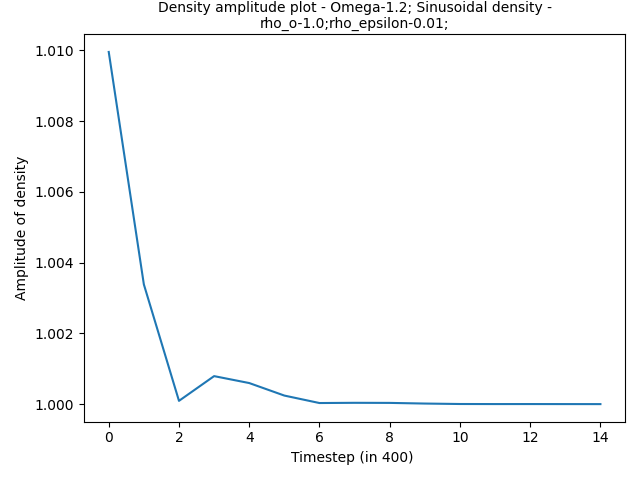
\includegraphics[width=\linewidth]{HPC_report/images/shear_wave_decay/sinusoidal_density/Amplitude-Timestep (in 400) -Amplitude of density.png}
        \caption{Amplitude of density along the Y-axis}
    \end{subfigure}
    \begin{subfigure}{0.3\textwidth}
        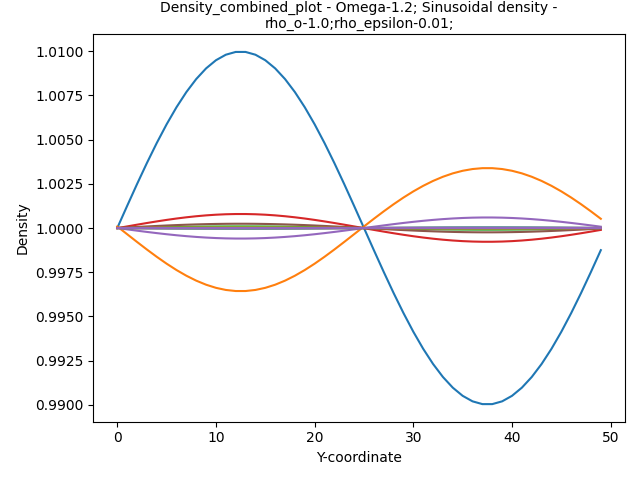
\includegraphics[width=\linewidth]{HPC_report/images/shear_wave_decay/sinusoidal_density/Combined_plot-Y-coordinate-Density.png}
        \caption{Time evolution of density}
    \end{subfigure}
    \begin{subfigure}{0.3\textwidth}
        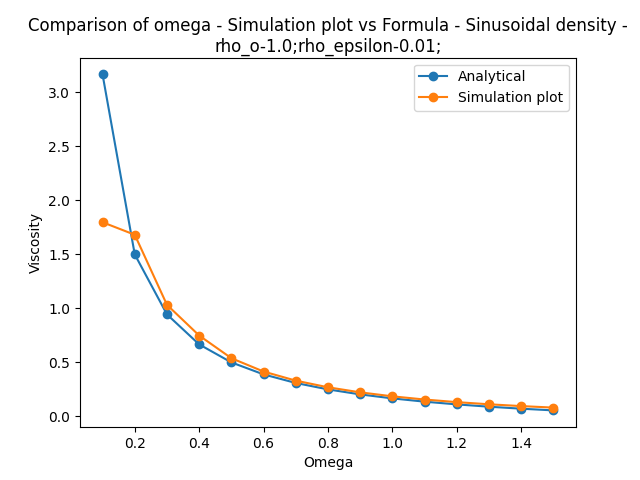
\includegraphics[width=\linewidth]{HPC_report/images/shear_wave_decay/Omega_comparison_Sinusoidal density_0.1_1.5_15.png}
        \caption{Analytical vs simulated viscosity}
        \label{fig:d_ac}
    \end{subfigure}
    \caption{Values for x=50 in lattice grid size 100x100 with configuration $\omega = 1.2$, Sinusoidal density with $\varepsilon = 0.01$ and Periodic Boundary Conditions}
\end{figure} 

\subsection{Couette Flow}
Couette flow describes fluid flow between a moving wall and a rigid wall. This section emphasizes the understanding of rigid and moving walls in the Lattice Boltzmann method. The top boundary is modelled as a moving wall with velocity $u_x$ and the bottom boundary is a rigid wall. Positive values of $u_x$ indicate that the wall is moving to the right. Periodic Boundary Conditions are applied at the left and right boundaries. The initial configuration ($t=0$) is as follows,

\begin{equation}
    \begin{aligned}
        \rho \left(0\right) &= 1.0 \\
        \mathbf{u} \left(0\right) &= 0
    \end{aligned}
    \label{eq:inital_config_default}
\end{equation}

\begin{figure}[h!]
  \begin{subfigure}{\textwidth}
        \centering
        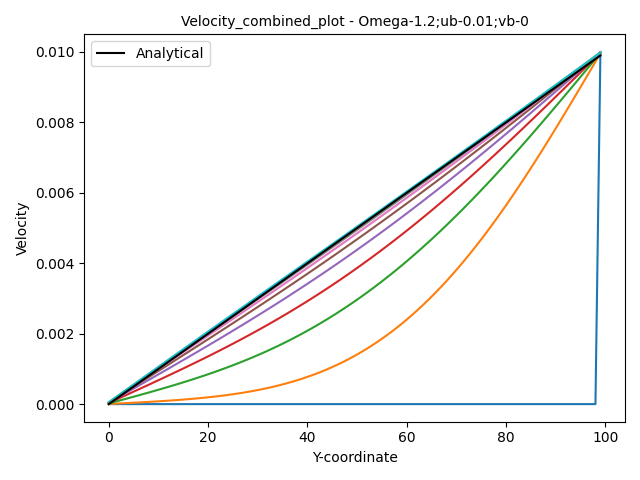
\includegraphics[width=0.4\linewidth]{HPC_report/images/couette/Combined_plot-Y-coordinate-Velocity.png}
        \caption{Time evolution of velocity along the Y-axis.}
        \label{fig:couette_velocity}
    \end{subfigure}
    \begin{subfigure}{\textwidth}
        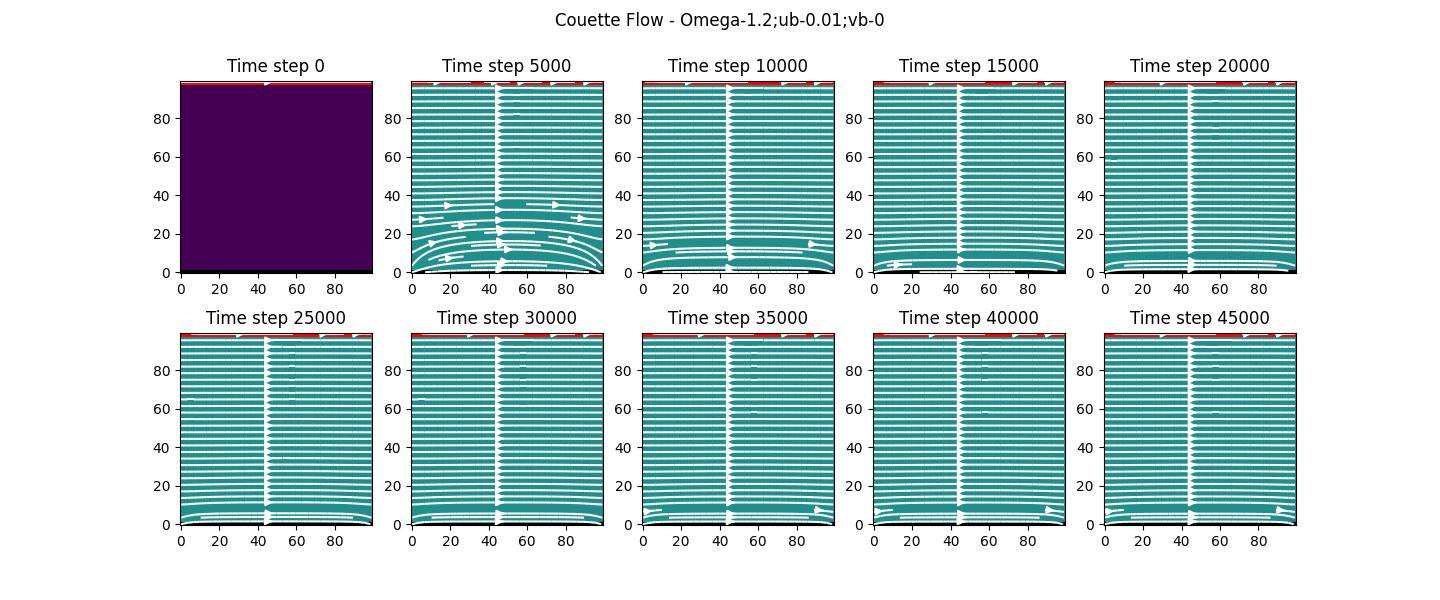
\includegraphics[width=\linewidth]{HPC_report/images/couette/Streamplot.png}
        \caption{Time evolution of density plot with velocity streamlines.}
    \end{subfigure}
    \caption{Couette Flow in lattice grid size 100x100 with configuration $\omega = 1.2$, Moving wall on top boundary (Colour red) with $u_x$=0.01, Rigid wall on bottom boundary (Colour black) and Periodic Boundary Conditions on the left and right boundaries. }
\end{figure} 

At $t \rightarrow \infty$, the velocity profile becomes stable, maintaining a consistent pattern. The fluid layers on top move with velocity close to that of the moving wall, while the fluid layers at the bottom are close to stagnant. Figure \ref{fig:couette_velocity} shows the velocity profile evolving from the initial configuration to the stable state.

The analytical solution for the velocity can be calculated as follow, \cite{CF_NagyGyrgy2018AGT}
\begin{equation}
    u\left(y\right) = \frac{y}{L_y} u_x
\end{equation}
where $L_y$ is the length of the grid along Y-axis. This velocity is plotted against the simulation values in Figure \ref{fig:couette_velocity}.

\subsection{Poiseuille Flow}
Poiseuille Flow models the fluid flow in a pipe characterized by pressure difference between the inlet and outlet. The top and bottom boundary are rigid walls with bounce back boundary conditions and the left and right boundaries have Periodic Boundary Conditions. Pressure gradients are implemented as a difference in density according to Equation \ref{eq:pressure_density}. The initial configuration is the same as Equation \ref{eq:inital_config_default}. In addition $\rho_{in}$ and $\rho_{out}$ are defined such that $\Delta \rho = \rho_{in} - \rho_{out}$ is of the order $10^{-3}$. Here, $\rho_{in} = 1.001$, and $\rho_{out} = 0.999$. This implementation is to experiment with pressure gradient based boundary conditions.

As $t \rightarrow \infty$, the velocity profile becomes stable, with the center of the pipe (Can be imagined as a line passing through the pipe equidistant from the rigid walls) having the maximum velocity and the fluid close to the rigid walls of the pipe having close to zero velocity. 

\begin{figure}[h!]
\begin{subfigure}{\textwidth}
    \begin{subfigure}{0.5\textwidth}
        \centering
        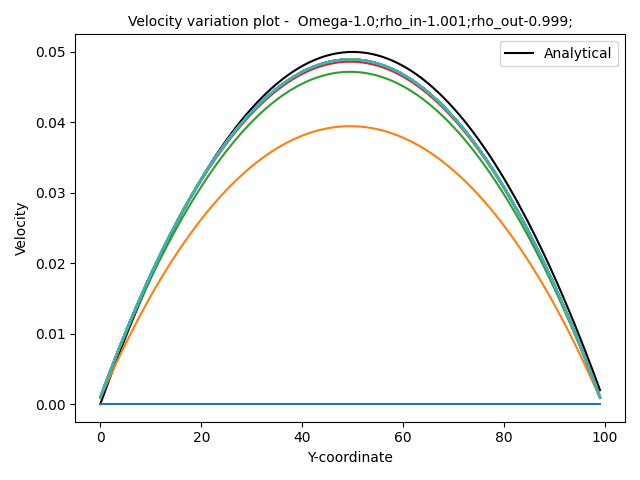
\includegraphics[width=0.8\linewidth]{HPC_report/images/poiseuille/o1/Combined_plot-Y-coordinate-Velocity.png}
        \captionsetup{font=small}
        \caption{Time evolution of velocity along the Y-axis at X=50 ($\omega = 1.0$)}
        \label{fig:p_velocity}
    \end{subfigure}
    \begin{subfigure}{0.5\textwidth}
        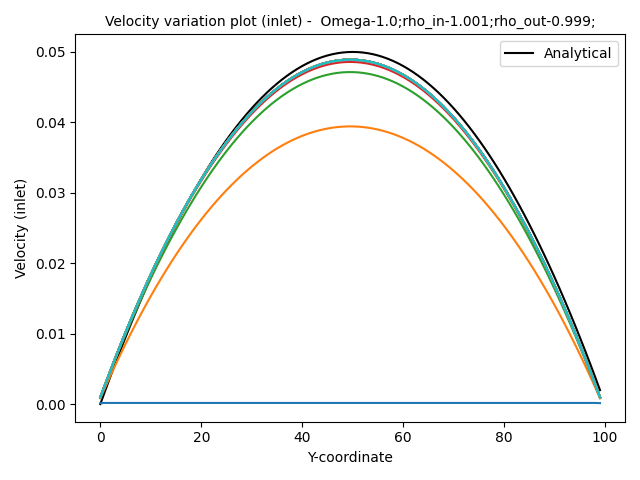
\includegraphics[width=0.8\linewidth]{HPC_report/images/poiseuille/o1/Combined_plot-Y-coordinate-Velocity (inlet).png}
        \captionsetup{font=small}
        \caption{Time evolution of velocity along the Y-axis at X=0 (Inlet) ($\omega = 1.0$)}
        \label{fig:p_velocity_inlet}
    \end{subfigure}
\end{subfigure}
\begin{subfigure}{\textwidth}
    \begin{subfigure}{0.5\textwidth}
        \centering
        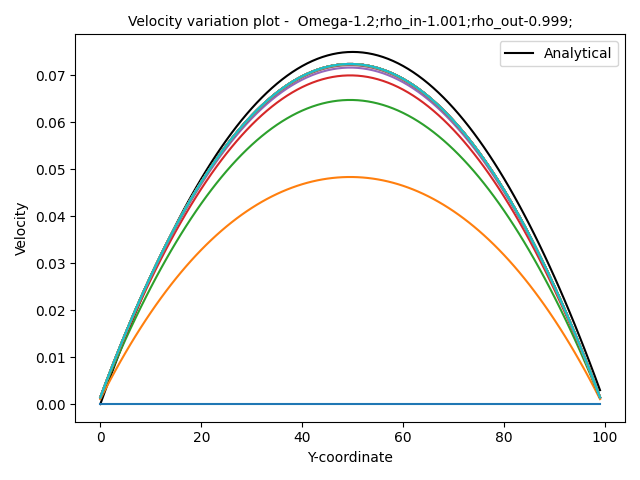
\includegraphics[width=0.8\linewidth]{HPC_report/images/poiseuille/o12/Combined_plot-Y-coordinate-Velocity.png}
        \captionsetup{font=small}
        \caption{Time evolution of velocity along the Y-axis at X=50 ($\omega = 1.2$)}
        \label{fig:p_velocity_2}
    \end{subfigure}
    \begin{subfigure}{0.5\textwidth}
        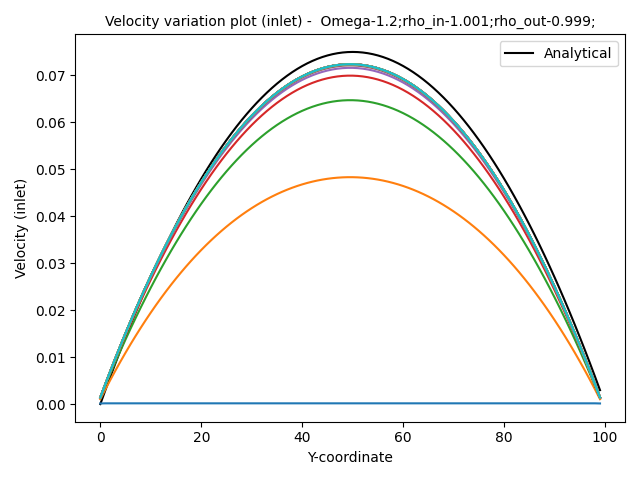
\includegraphics[width=0.8\linewidth]{HPC_report/images/poiseuille/o12/Combined_plot-Y-coordinate-Velocity (inlet).png}
        \captionsetup{font=small}
        \caption{Time evolution of velocity along the Y-axis at X=0 (Inlet) ($\omega = 1.2$)}
        \label{fig:p_velocity_inlet_2}
    \end{subfigure}
\end{subfigure}
    \caption{Poiseuille Flow in lattice grid size 100x100 with configuration Rigid wall on top and bottom boundary (Colour black) and Pressure gradient on the left and right boundaries with $\rho_{in}=1.001$ at the inlet and $\rho_{out}=0.999$ at the outlet. }
\end{figure} 

The velocity profile can also be calculated using the Navier-Stokes equation under the assumption of laminar flow. \cite{PF_Mendiburu2009ANALYTICALSF} Streaming velocity only has an X-component that is aligned with the axis of the pipe (Equation \ref{eq:navier-poiseuille}. Integrating along the wall normal direction and using boundary conditions $u(0)=0$ and $u(h)=0$, the velocity profile is given in Equation

\begin{equation}
    \frac{\partial p \left( x \right)} {\partial t} = \frac1 \mu \frac{\partial^2 u_x \left( y \right)} {\partial y^2}
    \label{eq:navier-poiseuille}
\end{equation}

\begin{equation}
    u \left( y \right) = - \frac{1}{2 \mu} \frac{dp}{dx} y \left(h-y\right)
\end{equation}
where $h$ is the diameter of the pipe (here, $ny$) and dynamic viscosity $\mu=\rho\nu$. The partial derivative is replaced by a total derivative as pressure only depends on the x-coordinate.

This analytical velocity is plotted against the time evolution of velocity through simulation. Figure \ref{fig:p_velocity} compares it to velocity profile generated at the midpoint of the length of the pipe $(X = \frac{nx}{2})$ and Figure \ref{fig:p_velocity_inlet} compares it to the velocity profile generated at the inlet $(X = 0)$. The velocity profile at the inlet and midpoint of the pipe length are visually identical. This correlates the laminar flow assumption. The plots also show that the stable velocity profile is closer to the analytical value as $\omega$ decreases.

\section{Sliding Lid}
Sliding Lid induced cavity is modelled by an enclosed fluid with a moving lid. The top boundary is a moving wall with velocity $u_x$ and the other three boundaries are rigid walls with bounce back conditions. The initial configuration is the same as Equation \ref{eq:inital_config_default}. In addition, the velocity of the moving wall is given by $u_x$ and positive values of $u_x$ indicate that the wall is moving to the right.

As $t \rightarrow \infty$, the vortexes formed stabilize and are different based on the initial configuration of the simulation.

\begin{figure}[h!]
  \begin{center}
   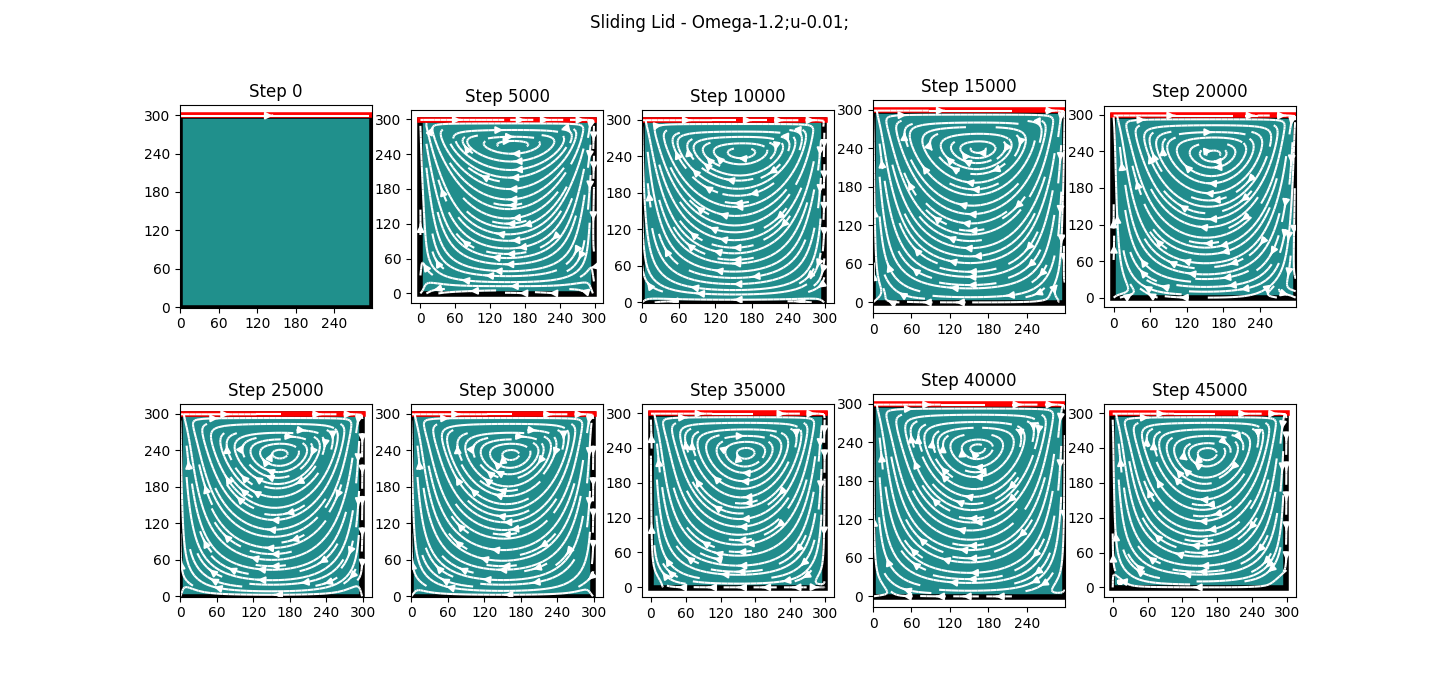
\includegraphics[width=\textwidth]{HPC_report/images/sliding_lid/Streamplot.png}
   \caption{Sliding Lid - Time evolution of density at x=150 in lattice grid size 300x300 with configuration $\omega = 1.2$, Moving wall at the top boundary (Colour Red) with $u_x$=0.01 and Rigid walls with bounce back (Colour Black) on left, right and bottom boundaries. Re = 27}
  \label{fig:sl_stream}
  \end{center}
\end{figure} 


\section{Flow patterns analysis with different Reynolds number}
The sliding lid on an enclosed fluid induces vortexes in the fluid that are characterized by a dimensionless entity called the \textbf{Reynolds Number (Re)}. 

The Reynolds number (Re) is a dimensionless quantity that characterizes the flow behavior of a fluid. It depends on the viscosity, density, velocity, and characteristic length of the enclosure. A higher value of Re $(> 2000)$ indicates fluid flow shifting towards turbulence. \cite{Re_Chiang1998EffectOR}

\begin{equation}
    Re = \frac{Lu}{\nu}
\end{equation}
$L$ is the length of the moving wall, $u$ is the velocity and $\nu$ is the kinematic viscosity that can be calculated from $\omega$ by Equation \ref{eq:viscosity}. $Lu$ represent the inertial terms and $\nu$ represents the viscous terms.

In this section, the sliding lid induced cavity is simulated for Re ranging from 100 to 1000 by varying different parameters of the initial configuration.

\subsection{Varying velocity}
The velocity of the moving wall on the top boundary is varied to achieve Re from 100 to 1000. The length and $\omega$ (and thus viscosity) are constant. The lattice grid of size $1000\times1000$ is initialized with $\omega = 1.2$ and $u_x$ varying from $0.01$ to $0.11$. The simulations are run for 50000 time steps.

\begin{figure}[h!]
  \begin{center}
   \includegraphics[width=\textwidth]{HPC_report/images/Re/Reynolds number comparison with varying velocity (L- 1000; Ω- 1.2).png}
   \caption{Sliding Lid - Snapshot of density of lattice grid size 1000x1000 with configuration $\omega = 1.2$, Moving wall at the top boundary (Colour Red) with $u_x$ varying from 0.01 to 0.11 (thus generating Re from 100 to 1000), and Rigid walls with bounce back (Colour Black) on left, right and bottom boundaries.}
  \label{fig:re_velocity}
  \end{center}
\end{figure} 

\subsection{Varying omega}
The omega value determines the kinematic viscosity by Equation \ref{eq:viscosity}. The omega is varied between 0.5 and 1.54 to achieve Re between 100 and 1000. The lattice grid of size $1000\times1000$ is initialized with $u_x$ = 0.5 and varying omega values. The simulations are run for 50000 time steps.

\begin{figure}[h!]
  \begin{center}
   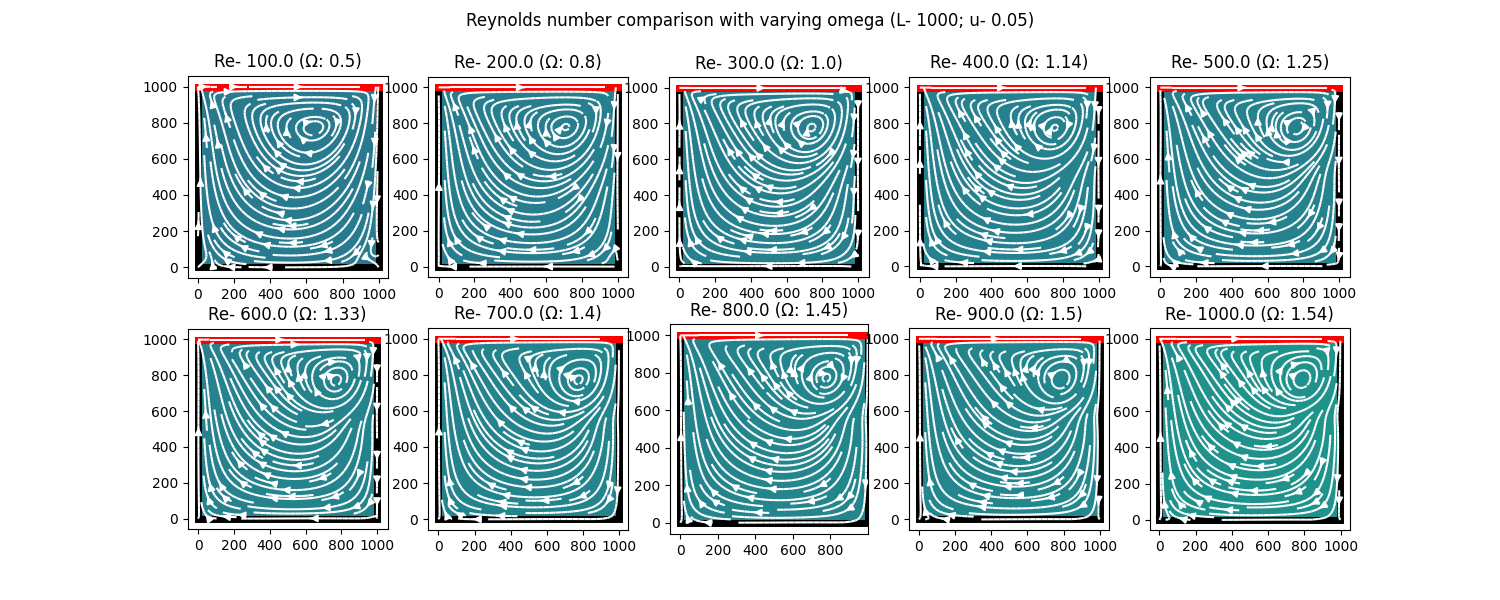
\includegraphics[width=\textwidth]{HPC_report/images/Re/Reynolds number comparison with varying omega (L- 1000; u- 0.05).png}
   \caption{Sliding Lid - Snapshot of density of lattice grid size 1000x1000 with configuration $\omega$ varying from 0.5 to 1.54 (thus generating Re from 100 to 1000), Moving wall at the top boundary (Colour Red) with $u_x$ = 0.05, and Rigid walls with bounce back (Colour Black) on left, right and bottom boundaries.}
  \label{fig:re_omega}
  \end{center}
\end{figure} 

\section{Scaling with processors}
In this section, the performance of the parallelized simulation is observed by running on different number of processors. For each execution, the time of execution is measured and MLUPS is calculated. MLUPS (Million Loops Per Second) is a measure of the computational efficiency in loop-intensive operations.

\begin{equation}
    MLUPS = \frac{Total Loops} {Execution Time * 10^6}
\end{equation}

The sliding lid induced cavity is simulated with three grid sizes $100\times100$, $500\times500$, $1000\times1000$. They are initialized with $\omega=1.2$ and moving wall on the top boundary with $u_x = 0.01$ while the three other boundaries are rigid walls with bounce back conditions. The number of processors range from 1 to 2500 in uneven intervals to accommodate splitting between the grid sizes.

All the scaling test experiments are performed on bwUniCluster \footnote{The authors acknowledge support by the state of Baden-Württemberg through bwHPC. 
 \url{https://wiki.bwhpc.de/e/Category:BwUniCluster_2.0}}.

\begin{figure}[h!]
  \begin{center}
   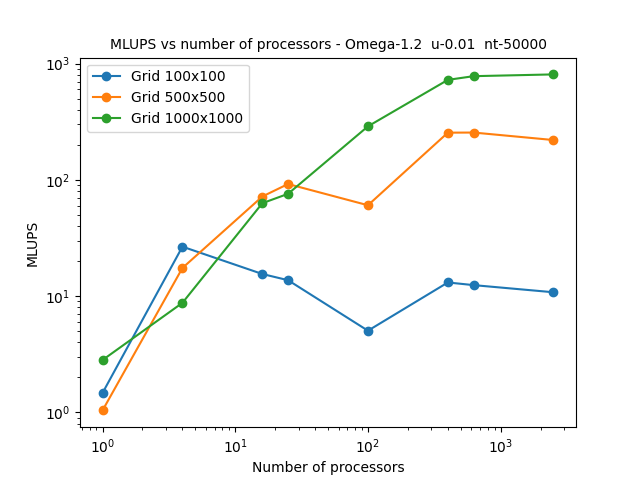
\includegraphics[width=0.8\textwidth]{HPC_report/images/sliding_lid/Plot_MLUPS.png}
   \caption{Sliding Lid induced cavity - Plot of MLUPS vs Number of processors for different grid sizes with configuration $\omega=1.2$, Moving wall at the top boundary (Colour Red) with $u_x$ = 0.01, and Rigid walls with bounce back (Colour Black) on left, right and bottom boundaries simulated for 50000 time steps.}
  \label{fig:mlups}
  \end{center}
\end{figure} 

The optimal number of processors for execution scales with the size of the lattice grid. Higher processor counts work well for larger grids. Performance degrades as the number of processors increases due to the latency of the communication and time lag in synchronization between the sub-domains. This is in line with Amdahl's Law.


\chapter{Conclusion}
The report starts by introducing the Lattice Boltzmann Method and motivating the need for High Performance Computing in the field of fluid dynamics. The idea of Python for HPC is also discussed.

Chapter 2 talks about the theoretical aspects of the Lattice Boltzmann Method and discretized equations for the same. The different components of the method including the mathematical elements required when simulating are explained. Multiple boundary condition options like Periodic Boundary Conditions, Rigid wall, Moving wall and Pressure gradients are introduced.

Chapter 3 discusses the implementation details including visualization techniques, packages and overall workflow of each of the simulations. The parallelization approach using spatial domain decomposition and MPI are explained.

Chapter 4 delves into the results for the simulation. The experiments are performed incrementally, starting from Shear Wave Decay with only PBC, followed by Couette flow with one moving and one rigid wall. Pressure gradient boundaries are also tested with Poiseuille Flow to deepen the understanding of the LBM. Finally, the Sliding Lid induced cavity is implemented in serial. With confidence in the accuracy of the simulation code, the experiment is parallelized and run on bwUniCluster \footnote{The authors acknowledge support by the state of Baden-Württemberg through bwHPC. 
 \url{https://wiki.bwhpc.de/e/Category:BwUniCluster_2.0}} for different configurations to observe the flow pattern variations. Scaling tests were also done across a range of processor counts to assess performance. The optimal number of processors for execution scales with the size of the lattice grid but the performance degrades as the number of processors increases in line with Amdahl's Law due to communication overhead.
 

\bibliographystyle{unsrt}
\bibliography{biblio}

\end{document}
